\newpage
\subsection{Examenvragen hoofdstuk 8}

\begin{enumerate} %opsomming 1

    \item Leg volgende bewering uit: IPsec is een veiligheidsdeken.
Veiligheidsdeken = blanket coverage.

    \enumeratext{Zie hoofdstuk 8 pagina 666 – 668 en slides 81 – 90.}

    \item Een hashfunctie is veiliger dan een checksom.
    
\enumeratext{test invullen}

    \item Als netwerkbeheerder bij ICMP-ZERO moet je de firewall configureren zodat de DMZ niet kan gemapt worden door middel van traceroute. Teken deze configuratie en schrijf in pseudocode de FW-regels.
    
\enumeratext{test invullen}

\item Het verschil tussen ECB en CBC en waarom dat het een beter is dan het andere

%\enumeratext{} zorgt ervoor dat je tekst kan typen tussen lijstitems in
\enumeratext{Cipher Block Chaining}

\item Kan er gezegd worden dat een CA een "Thrusted Thirth Party" is bij PKI

\enumeratext{test invullen}

\item Leg onweerlegbaarheid uit bij het gebruik van PGP

\enumeratext{test invullen}

\item Hoe werkt pgp en hoe garandeert het integriteit en authenticatie? Leg uit Onweerlegbaarheid/Non-repudiation

\enumeratext{test invullen}

\item Het belang van een nonce binnen authenticatie
Nonce = een nummer (R) dat maar 1 keer mag gebruikt worden. (= once-in-a-lifetime)

\enumeratext{test invullen}

\item Wat is de cryptografische functie een CA

\enumeratext{test invullen}

\item Bob en Alice hebben elk een publieke sleutel, twee manier geven hoe dat Trudy deze niet kan onderscheppen

\enumeratext{test invullen}

\item Uitleggen bij een packet filter en een inspection firewall hoe dat je die kunt omzeilen als je gebruik maakt van passive ftp

\enumeratext{test invullen}

\item Waarom is een gedistribueerde hashtabel een 'HASH'-tabel?

\enumeratext{test invullen}

\item Leg volgende begrippen uit aan de hand van een schema (schema moet je zelf tekenen) : intern net, demiliteraized zone, firewall, router, webserver.

\enumeratext{test invullen}

\item Plaats een ACL waarbij enkel inkomende verbindingen op poort 80 geaccepteerd worden op het schema om de webserver beter te beveiligen.

\enumeratext{test invullen}

\item Geef 2 algoritmes waarbij het niet belangrijk is dat de data geheim is. Leg beide kort uit.

\enumeratext{test invullen}

\item Geef een voorbeeld van een service die met UDP werkt en wat zijn de voordelen hiervan.

\enumeratext{test invullen}

\item Alice wil veilig communiceren met Bob via zijn publieke sleutel. Hoe kan ze zeker zijn dat ze met Bob communiceert en niet met Trudy die de pakketten probeert te onderscheppen. Geef twee manieren hoe de uitwisseling veilig kan gebeuren en leg kort uit.

\enumeratext{test invullen}

\item Wat zijn de voor- en nadelen van zowel symmetrische als asymmetrische encryptie. Hoe kan men deze het beste combineren.

\enumeratext{test invullen}

\item Indien Alice contact wilt maken met Bob. Hoe kan ze er dan voor zorgen dat Trudy niet als 'man in the middle' fungeert. En dus haar publieke sleutel aan Alice doorgeeft en doet alsof ze Bob is.

\enumeratext{test invullen}

\item Cipher Block Chaining: wat is het?

\enumeratext{test invullen}

\item Diffie-Hellman in schemavorm uitleggen. Hoe kan je daar misbruik van maken (Man In The Middle).

\enumeratext{test invullen}

\item PGP in schema: wat gebeurt er als je de hash wegdoet, is dan integriteit en confidentialiteit en authenticiteit nog in orde? Wat is er symmetrisch en assymetrisch aan? Wat kan Trudy doen om toch de boodschap teweten te komen en wat is de oplossing (certificaten gebruiken)?

\enumeratext{test invullen}

\item Wat is PGP? Hoe zorgt dit voor integriteit en authenticatie?

\enumeratext{test invullen}

\item Wat is een digitale handtekening? Hoe zorgt dit voor integriteit en authenticiteit.

\enumeratext{test invullen}

\clearpage

\item	waar of niet waar + leg uit (hierop krijg je punten)
    \begin{enumerate} %opsomming 2
        \item Het Diffie-Hellman algoritme is een hashfunctie.

\enumeratext{test invullen}

        \item Een hashfunctie is veiliger dan een checksom.

\enumeratext{test invullen}

        \item Als een hacker de Publieke Sleutel van een website in handen krijgt heeft deze toegang tot alle sessies, en alle voorgaande sessies als deze werden opgenomen (Sniffing)

\enumeratext{test invullen}

        \item Als een hacker de Private Sleutel van een website in handen krijgt heeft deze toegang tot alle sessies, en alle voorgaande sessies als deze werden opgenomen (Sniffing)?

\enumeratext{test invullen}

        \item Een Packet-filter kan geen virussen tegenhouden

\enumeratext{test invullen}

        \item In een DMZ (Demilitarized Zone) staan geen interne servers

\enumeratext{test invullen}

        \item Een systeem dat gebruikt maakt van HMAC is gevoelig voor replayaanvallen

\enumeratext{test invullen}

        \item Als bij een diefstal de Private Sleutel van een Certification Authency (CA) gestolen wordt, heeft dit dan invloed op vooraf uitgedeelde certificaten door deze sleutel?

\enumeratext{test invullen}

        \item Zonder CBC is bij AES niet mogelijk om afbeeldingen te beveiligen

\enumeratext{test invullen}

        \item Door de komst van asymmetrische sleutels zijn symmetrische sleutels eigenlijk niet meer nuttig.

\enumeratext{test invullen}

        \item Een IPSEC AH (Authentication Header) zorgt ervoor dat de header van een IP-pakket niet meer veranderd kan worden door een digitale handtekening.

\enumeratext{test invullen}

        \item Een wiskundige vindt een snelle manier om een product in 2 priemgetallen op te splitsen, is het RSA in gevaar?

\enumeratext{test invullen}

        \item Het Session Initiation Protocol dient om media (audio/video) te versturen

\enumeratext{test invullen}

        \item SSL wordt gebruikt bij HTTPS
                

\enumeratext{Correct.}
                
        \item Bij HTTPS wordt alles met het certificaat van de server versleutelt

\enumeratext{test invullen}

        \item NAT werkt niet met IPsec (AH) in tunnelmode , met esp wel

\enumeratext{test invullen}

        \item DMZ is enkel beveiligd door controle van de router, op elke server moet nog beveiliging opkomen, op DMZ moet de buitenwereld op kunnen, op het bedrijfsnetwerk niet en is dus beter beschermd. Wel kan een firewall die meer als 2 interfaces gebruikt ook de DMZ beveiligen

\enumeratext{test invullen}

        \item De routetabellen van de AS'en worden manueel bijgewerkt wrong... routetabellen worden up-to-date gehouden door dat ze naar elkaar berichten zetten die voldoen aan het BGP (inmiddels versie 4)

\enumeratext{test invullen}

        \item PGP heeft certificaten en genereert een zogenaamde digitale vingerafdruk die kan gebruikt worden om na te gaan of een gebruiker echt is

\enumeratext{test invullen}


        \item Via een certificaat is de eindgebruik zeker dat de server waarmee hij verbinding heeft gemaakt effectief de gevraagde server (en houder van het certificaat) is.
        
%\enumeratext{r}

        \end{enumerate} %einde opsomming 2
 
\item	Termen uitleggen

    \begin{enumerate} %opsomming 3
    
        \item http hijacking

\enumeratext{test invullen}

        \item FTP in passive mode

\enumeratext{test invullen}

        \item VPN

\enumeratext{test invullen}

        \item Ticket (Kerberos)

\enumeratext{test invullen}

        \item Diffie Helman

\enumeratext{test invullen}

        \item Internet exchange

\enumeratext{test invullen}


        \item ACL (Access Control List)

\enumeratext{test invullen}

        \item PGP

\enumeratext{test invullen}

        \item DMZ

\enumeratext{test invullen}

        \item Signature-based IDS (Intrusion Detection System)

\enumeratext{test invullen}

        \item Tunnel en transport mode bij IPSec
        
%\enumeratext{}

    \end{enumerate} %einde opsomming 3
    
  \end{enumerate} %einde opsomming 1
  
\subsection{vragen uit boek van hoofdstuk 8}

\noindent SECTION 8.1

\begin{enumerate}

\item  What are the differences between message confidentiality and message integrity? Can you have confidentiality without integrity? Can you have integrity without confidentiality? Justify your answer.

\enumeratext{Confidentiality is the property that the original plaintext message can not be determined by an attacker who intercepts the ciphertext-encryption of the original plaintext message. Message integrity is the property that the receiver can detect whether the message sent (whether encrypted or not) was altered in transit. The two are thus different concepts, and one can have one without the other. An encrypted message that is altered in transmit may still be confidential (the attacker can not determine the original plaintext) but will
not have message integrity if the error is undetected. Similarly, a message that is altered in transit (and detected) could have been sent in plaintext and thus would not be confidential.}


\item Internet entities (routers, switches, DNS servers, Web servers, user end systems, and so on) often need to communicate securely. Give three specific example pairs of Internet entities that may want secure communication.

\enumeratext{(i) User’s laptop and a web server; (ii) two routers; (iii) two DNS name servers. }

\end{enumerate}

\noindent SECTION 8.2

\begin{enumerate}

\item From a service perspective, what is an important difference between a symmetric-key system and a public-key system?

\enumeratext{One important difference between symmetric and public key systems is that in symmetric key systems both the sender and receiver must know the same (secret) key. In public key systems, the encryption and decryption keys are distinct. The encryption key is known
by the entire world (including the sender), but the decryption key is known only by the receiver.}

\item Suppose that an intruder has an encrypted message as well as the decrypted version of that message. Can the intruder mount a ciphertext-only attack, a known-plaintext attack, or a chosen-plaintext attack?

\enumeratext{In this case, a known plaintext attack is performed. If, somehow, the message encrypted by the sender was chosen by the attacker, then this would be a chosen-plaintext attack.}

\item Consider an 8-block cipher. How many possible input blocks does this cipher have? How many possible mappings are there? If we view each mapping as a key, then how many possible keys does this cipher have?

\enumeratext{An 8-block cipher has $2^8$ possible input blocks. Each mapping is a permutation of the $2^8$ input blocks; so there are $2^8 !$ possible mappings; so there are $2^8 !$ possible keys}

\item Suppose N people want to communicate with each of N – 1 other people using symmetric key encryption. All communication between any two people, i and j, is visible to all other people in this group of N, and no other person in this group should be able to decode their communication. How many keys are required in the system as a whole? Now suppose that public key encryption is used. How many keys are required in this case?

\enumeratext{If each user wants to communicate with N other users, then each pair of users must have a shared symmetric key. There are N*(N-1)/2 such pairs and thus there are N*(N-1)/2 keys. With a public key system, each user has a public key which is known to all, and a
private key (which is secret and only known by the user). There are thus 2N keys in the public key system.}

\item Suppose n = 10,000, a = 10,023, and b = 10,004. Use an identity of modular arithmetic to calculate in your head (a • b) mod n.

\enumeratext{ a mod n = 23 , b mod n = 4. So (a*b) mod n = 23*4=92}

\item Suppose you want to encrypt the message 10101111 by encrypting the decimal number that corresponds to the message. What is the decimal number?

\enumeratext{answer: 175}

\end{enumerate}

\noindent SECTIONS 8.3–8.4

\begin{enumerate}

\item In what way does a hash provide a better message integrity check than a checksum (such as the Internet checksum)?

\enumeratext{One requirement of a message digest is that given a message M, it is very difficult to find another message M’ that has the same message digest and, as a corollary, that given a message digest value it is difficult to find a message M’’ that has that given message
digest value. We have “message integrity” in the sense that we have reasonable confidence that given a message M and its signed message digest that the message was not altered since the message digest was computed and signed. This is not true of the
Internet checksum, where we saw in Figure 7.18 that it easy to find two messages with the same Internet checksum}

\item Can you “decrypt” a hash of a message to get the original message? Explain your answer.

\enumeratext{No. This is because a hash function is a one-way function. That is, given any hash value, the original message cannot be recovered (given h such that h=H(m), one cannot recover m from h).}

\item Consider a variation of the MAC algorithm (Figure 8.9) where the sender sends (m, H(m) + s), where H(m) + s is the concatenation of H(m) and s. Is this variation flawed? Why or why not?

\enumeratext{This is scheme is clearly flawed. Trudy, an attacker, can first sniff the communication and obtain the shared secret s by extracting the last portion of digits from H(m)+s. Trudy can then masquerade as the sender by creating her own message t and send (t, H(t)+s).}

\item What does it mean for a signed document to be verifiable and non-forgeable?

\enumeratext{ Suppose Bob sends an encrypted document to Alice. To be verifiable, Alice must be able to convince herself that Bob sent the encrypted document. To be non-forgeable, Alice must be able to convince herself that only Bob could have sent the encrypted document
(e.g.,, non one else could have guess a key and encrypted/sent the document) To be nonreputiable, Alice must be able to convince someone else that only Bob could have sent the document. To illustrate the latter distinction, suppose Bob and Alice share a secret
key, and they are the only ones in the world who know the key. If Alice receives a document that was encrypted with the key, and knows that she did not encrypt the document herself, then the document is known to be verifiable and non-forgeable (assuming a suitably strong encryption system was used). However, Alice can not convince someone else that Bob must have sent the document, since in fact Alice knew
the key herself and could have encrypted/sent the document.}

\item In what way does the public-key encrypted message hash provide a better digital signature than the public-key encrypted message?

\enumeratext{A public-key signed message digest is “better” in that one need only encrypt (using the private key) a short message digest, rather than the entire message. Since public key encryption with a technique like RSA is expensive, it’s desirable to have to sign (encrypt)
a smaller amount of data than a larger amount of data.}

\item Suppose certifier.com creates a certificate for foo.com. Typically, the entire certificate would be encrypted with certifier.com’s public key. True or False?

\enumeratext{This is false. To create the certificate, certifier.com would include a digital signature, which is a hash of foo.com’s information (including its public key), and signed with certifier.com’s private key.}

\item Suppose Alice has a message that she is ready to send to anyone who asks. Thousands of people want to obtain Alice’s message, but each wants to be sure of the integrity of the message. In this context, do you think a MAC-based or a digital-signature-based integrity scheme is more suitable? Why?

\enumeratext{For a MAC-based scheme, Alice would have to establish a shared key with each potential recipient. With digital signatures, she uses the same digital signature for each recipient; the digital signature is created by signing the hash of the message with her private key. Digital signatures are clearly a better choice here.}

\item What is the purpose of a nonce in an end-point authentication protocol?

\enumeratext{The purpose of the nonce is to defend against the replay attack.}

\item What does it mean to say that a nonce is a once-in-a-lifetime value? In whose lifetime?

\enumeratext{Once in a lifetimes means that the entity sending the nonce will never again use that value to check whether another entity is “live”. }

\item Is the message integrity scheme based on HMAC susceptible to playback attacks? If so, how can a nonce be incorporated into the scheme to remove this susceptibility?

\enumeratext{ In a man-in-the-middle attack, the attacker puts himself between Alice and Bob, altering the data sent between them. If Bob and Alice share a secret authentication key, then any alterations will be detected.}

\end{enumerate}

\newpage

\noindent SECTIONS 8.5–8.8

\begin{enumerate}

\item Suppose that Bob receives a PGP message from Alice. How does Bob know for sure that Alice created the message (rather than, say, Trudy)? Does PGP use a MAC for message integrity?

\enumeratext{Alice provides a digital signature, from which Bob can verify that message came from Alice. PGP uses digital signatures, not MACs, for message integrity.}

\item  In the SSL record, there is a field for SSL sequence numbers. True or False?

\enumeratext{False. SSL uses implicit sequence numbers.}

\item What is the purpose of the random nonces in the SSL handshake?

\enumeratext{The purpose of the random nonces in the handshake is to defend against the connection
replay attack.}

\item Suppose an SSL session employs a block cipher with CBC. True or False: The server sends to the client the IV in the clear?

\enumeratext{True. The IV is always sent in the clear. In SSL, it is sent during the SSL handshake. }

\item Suppose Bob initiates a TCP connection to Trudy who is pretending to be Alice. During the handshake, Trudy sends Bob Alice’s certificate. In what step of the SSL handshake algorithm will Bob discover that he is not communicating with Alice?

\enumeratext{After the client will generate a pre-master secret (PMS), it will encrypt it with Alice’s public key, and then send the encrypted PMS to Trudy. Trudy will not be able to decrypt the PMS, since she does not have Alice’s private key. Thus Trudy will not be able to determine the shared authentication key. She may instead guess one by choosing a random key. During the last step of the handshake, she sends to Bob a MAC of all the handshake messages, using the guessed authentication key. When Bob receives the MAC, the MAC test will fail, and Bob will end the TCP connection.}

\item  Consider sending a stream of packets from Host A to Host B using IPsec. Typically, a new SA will be established for each packet sent in the stream. True or False?

\enumeratext{False. Typically an IPsec SA is first established between Host A and Host B. Then all packets in the stream use the SA.}

\item  Suppose that TCP is being run over IPsec between headquarters and the branch office in Figure 8.28. If TCP retransmits the same packet, then the two corresponding packets sent by R1 packets will have the same sequence number in the ESP header. True or False? 

\enumeratext{False. IPsec will increment the sequence number for every packet it sends.}

\item An IKE SA and an IPsec SA are the same thing. True or False?

\enumeratext{False. An IKE SA is used to establish one or more IPsec SAs. }

\end{enumerate}

\newpage

\noindent SECTION 8.9

\begin{enumerate}

\item  Stateful packet filters maintain two data structures. Name them and briefly describe what they do.

\enumeratext{Filter table and connection table. The connection table keeps track of connections, allowing for a finer degree of packet filtering.}

\item  Consider a traditional (stateless) packet filter. This packet filter may filter packets based on TCP flag bits as well as other header fields. True or False?

\enumeratext{TRUE}

\item In a traditional packet filter, each interface can have its own access control list. True or False?

\enumeratext{ TRUE}

\item Why must an application gateway work in conjunction with a router filter to be effective?

\enumeratext{If there isn’t a packet filter, than users inside the institution’s network will still be able to make direct connections to hosts outside the institution’s network. The filter forces the users to first connect to the application gateway. }

\item Signature-based IDSs and IPSs inspect into the payloads of TCP and UDP segments. True or False?

\enumeratext{ TRUE}

\end{enumerate}

\newpage

Problems

\begin{enumerate}
    \item Provide a filter table and a connection table for a stateful firewall that is as restrictive as possible but accomplishes the following:
    
    \begin{enumerate}
\item Allows all internal users to establish Telnet sessions with external
hosts.
\item Allows external users to surf the company Web site at 222.22.0.12.
\item But otherwise blocks all inbound and outbound traffic.
\item The internal network is 222.22/16. In your solution, suppose that the connection table is currently caching three connections, all from inside to outside. You’ll need to invent appropriate IP addresses and port numbers.

    \end{enumerate}

\enumeratext{

\begin{figure}[h]
    \centering
    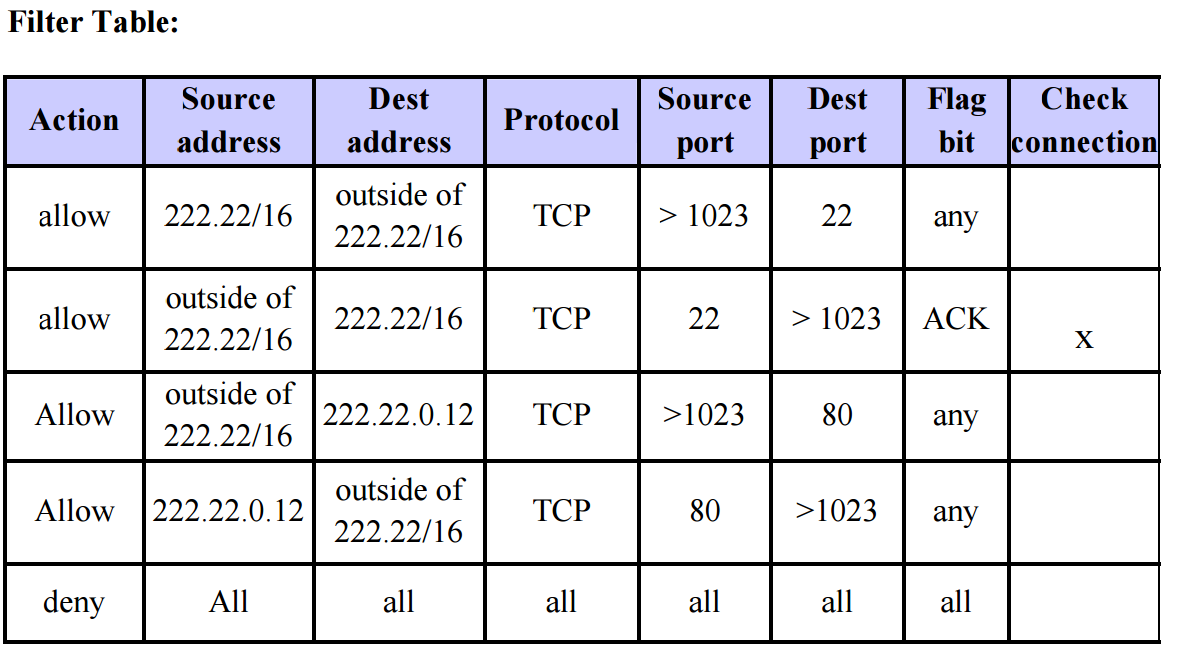
\includegraphics[width=7in]{./img/imghfdst8/answer1.PNG}
    \caption{Filter Table:  }      
    \label{fig:Filter Table:  }
\end{figure}


\begin{figure}[h]
    \centering
    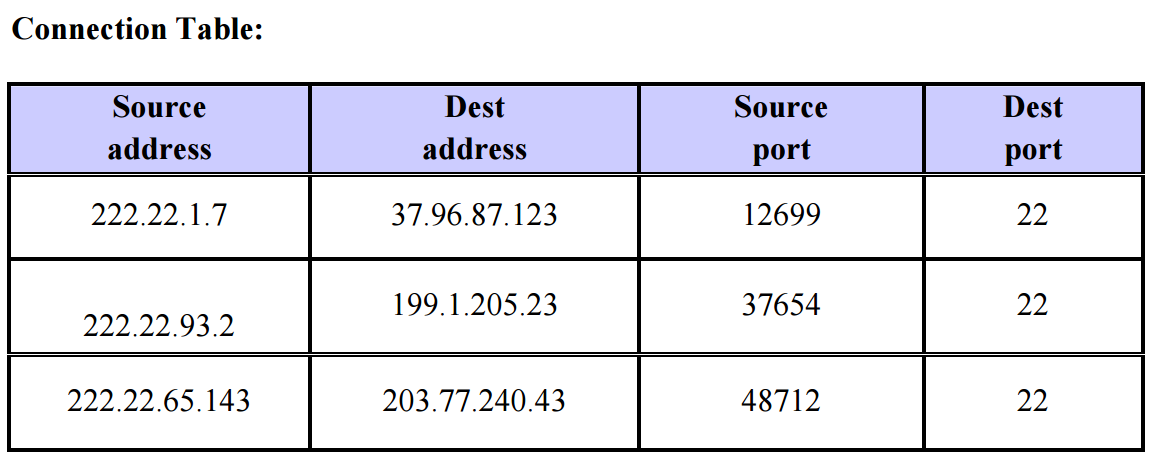
\includegraphics[width=7in]{./img/imghfdst8/answer2.PNG}
    \caption{Connection Table:  }      
    \label{fig:Connection Table: }
\end{figure}

}
\end{enumerate}



